%----------------------------------------------------------------------------------
% Exemplo do uso da classe tcc.cls. Veja o arquivo .cls
% para mais detalhes e instruções.
%----------------------------------------------------------------------------------

% Seleção de idioma da monografia. Por enquanto as únicas opções
% suportadas são 'portuguese' e 'english'
% Para impressão em frente e verso, use a opção 'twoside'. Da
% mesma forma, use 'oneside' para impressão em um lado apenas.
\documentclass[portuguese,oneside]{tcc}

%----------------------------------------------------------------
% Coloque seus pacotes abaixo.
%
% Obs.: muitos pacotes de uso comum do LaTeX, como amsmath,
% geometry e url já são automaticamente incluídos pela classe
% (veja o arquivo .cls). Isso torna obrigatória a presença destes
% no sistema para o uso desta classe, mas ao mesmo tempo o uso se
% torna mais simples.  Recomendo a instalação da versão mais
% recente da distribuição TeXLive (para Windows e UNIXes):
% www.tug.org/texlive/
%
% Pacotes e opções já incluídas automaticamente:
%
% \RequirePackage[T1]{fontenc}[2005/09/27]
% \RequirePackage[utf8x]{inputenc}[2008/03/30]
% \RequirePackage[english,brazil]{babel}[2008/07/06]
% \RequirePackage[a4paper]{geometry}[2010/09/12]
% \RequirePackage{textcomp}[2005/09/27]
% \RequirePackage{lmodern}[2009/10/30]
% \RequirePackage{indentfirst}[1995/11/23]
% \RequirePackage{setspace}[2000/12/01]
% \RequirePackage{textcase}[2004/10/07]
% \RequirePackage{float}[2001/11/08]
% \RequirePackage{amsmath}[2000/07/18]
% \RequirePackage{amssymb}[2009/06/22]
% \RequirePackage{amsfonts}[2009/06/22]
% \RequirePackage{url}
% \RequirePackage[table]{xcolor}[2007/01/21]
%----------------------------------------------------------------
% Para inserção de figuras.
\usepackage{graphicx}
% Utilize a opção 'pdftex' se você estiver usando o pdflatex (que
% permite figuras em formatos como .jpg ou .png)
%\usepackage[pdftex]{graphicx}

% Para tabelas com elementos ocupando mais de uma linha
\usepackage{multirow}
% Para frações na mesma linha (ex. ⅓).
\usepackage{nicefrac}
% Para inserir figuras lado a lado.
% \usepackage{subfigure}
% Para formatar algoritmos.
% A opção [algo2e] é necessária para evitar conflitos
% com as definições da classe.
%\usepackage[algo2e]{algorithm2e}
\usepackage{algorithmic}
% Um float do tipo algoritmo. No momento
% este pacote é incompatível com a classe.
%\usepackage{algorithm}

\usepackage{todonotes}

%----------------------------------------------------------------
% Autor (OBRIGATÓRIO)
%----------------------------------------------------------------
\author{Vinicius Jaggi}

%----------------------------------------------------------------
% Título (OBRIGATÓRIO). Devem ser passados DOIS parâmetros,
% o título em português E o inglês, não importando o idioma
% escolhido. Os títulos são utilizados para a montagem da capa,
% resumo e abstract mais tarde.
%----------------------------------------------------------------
\title{Adoção de práticas de segurança da ISO 27000  por desenvolvedores de Software Mobile}
     {Your title in english here}

%----------------------------------------------------------------
% Opções para o tipo de trabalho (OBRIGATÓRIO)
%----------------------------------------------------------------
%\tipotrabalho{\ptci}         % Proposta de Trabalho de Conclusão
\tipotrabalho{\tci}         % Trabalho de Conclusão I
%\tipotrabalho{\tcii}        % Trabalho de Conclusão II

%----------------------------------------------------------------
% Seleção do curso ("este trabalho é um requisito parcial parahttps://pt.overleaf.com/project/5e7df1075c75e20001f34b9f
% obtenção do grau de (mestre ou doutor) em Ciência da Computação").
%----------------------------------------------------------------
%\curso{\cc} % Ciência da Computação
\curso{\si} % Sistemas de Informação
%\curso{\es} % Engenharia de Software

%----------------------------------------------------------------
% Orientador (e Co-orientador, caso haja um). É OBRIGATÓRIO
% informar pelo menos o orientador.
%----------------------------------------------------------------
\orientador{MSc Azriel Majdenbaum}
\coorientador{PhD Sabrina Marczak}


%----------------------------------------------------------------
% A capa é inserida automaticamente. Por isso não é necessário
% chamar \maketitle
%----------------------------------------------------------------
\begin{document}

%----------------------------------------------------------------
% Depois da capa vem a dedicatória e a epígrafe.
%----------------------------------------------------------------
%\dedicatoria{Dedico este trabalho a meus pais.}

%\epigrafe{The art of simplicity is a puzzle of complexity.}
         %{Douglas Horton}

%----------------------------------------------------------------
% Também dá para fazer as duas na mesma página:
%----------------------------------------------------------------
%\dedigrafe{Dedico este trabalho a meus pais.}
%          {The art of simplicity is a puzzle of complexity.}
%          {Douglas Horton}

%----------------------------------------------------------------
% A seguir, a página de agradecimentos (OPCIONAL):
%----------------------------------------------------------------
%\begin{agradecimentos}
%AGRADECIMENTOS AQUI
%\end{agradecimentos}

%----------------------------------------------------------------
% Resumo, com as palavras-chave passadas por parâmetro
% (OBRIGATÓRIO, ao menos para teses e dissertações)
%----------------------------------------------------------------
\begin{resumo}{Segurança da Informação,Família ISO 27000, ISO 27002, Controles de Segurança, Desenvolvimento \textit{mobile}, \textit{Survey}}

 A Segurança da Informação é uma área importante da computação que se vale de guias e padrões para garantir a segurança de sistemas de software. Por meio da norma ISO 27001, é possível elaborar um Sistema de Gerenciamento da Segurança da Informação que busca reduzir os riscos de vulnerabilidade que comprometam os ativos de informação. Adotar as especificações dessa norma é um desafio, seja pelo desconhecimento de sua importância ou pela falta de entendimento de seus controles. Este Trabalho de Conclusão de Curso visa identificar por meio de uma \textit{survey} quais são os controles da ISO 27002 adotados no desenvolvimento de \textit{software} \textit{mobile} e quais são as dificuldades ao tentar adotá-los, de forma a sugerir um conjunto de recomendações de uso para suprir essas dificuldades. Para se atingir o objetivo desde TCC, foi utilizada a revisão da literatura de Steglich e colegas \cite{caio2019} no tema como inspiração, estudou-se em profundidade os controles da ISO 27002 com o objetivo de selecionar os constructos de referência para a definição do questionário da \textit{survey} em questão. A seleção desses constructos, ou controles da ISO 27002, foram discutidos com três pesquisadores que acompanham este Trabalho e, como próximo passo, como primeira atividade do Trabalho de Conclusão II, serão validados com especialistas, em um estudo baseado em entrevistas. Os resultados da \textit{survey} servirão de base para a definição de um conjunto de recomendações para desenvolvedores \textit{mobile}, a serem disponibilizadas de forma online para consulta da comunidade.     
 


%Tendo conhecimento desses padrões ira se realizar um estudo utilizando a metodologia survey , com o objetivo de identificar os  controles da ISO 27.002 utilizados no desenvolvimento de software mobile e quais são as dificuldades de adotar tais padrões.


\end{resumo}

%----------------------------------------------------------------
% Abstract, com as palavras-chave passadas por parâmetro
% (OBRIGATÓRIO, ao menos para teses e dissertações)
%----------------------------------------------------------------
%\begin{abstract}{lorem, ipsum, dolor, sit, amet}
%ESCREVER AQUI O ABSTRACT
%\end{abstract}

%----------------------------------------------------------------
% Listas e sumário, nessa ordem. Somente o sumário é obrigatório,
% portanto, comente as outras listas, caso sejam desnecessárias.
%----------------------------------------------------------------
\listoffigures       % Lista de figuras      (OPCIONAL)
\listoftables        % Lista de tabelas      (OPCIONAL)
%\listofalgorithms    % Lista de algoritmos   (OPCIONAL)
\listofacronyms      % Lista de siglas       (OPCIONAL)
%\listofabbreviations % Lista de abreviaturas (OPCIONAL)
%\listofsymbols       % Lista de símbolos     (OPCIONAL)
\tableofcontents     % Sumário               (OBRIGATÓRIO)

%----------------------------------------------------------------
% Aqui começa o desenvolvimento do trabalho. Para uma melhor
% organização do documento, separe-o em arquivos,
% um para cada capítulo. Para isso, utilize o comando \include,
% como mostrado abaixo.
%----------------------------------------------------------------
%----------------------------------------------------------------------------------
% Exemplo do uso da classe tcc.cls. Veja o arquivo .cls
% para mais detalhes e instruções.
%----------------------------------------------------------------------------------
\chapter{\label{chap:intro}Introdução}
% Comando para inserir siglas. Tanto as siglas quanto as
% abreviaturas devem aparecer em ordem ALFABÉTICA nas listas
% correspondentes. Como a classe no momento não é capaz de ordenar
% as entradas automaticamente, existem duas alternativas:
%
%    a- Insira todas as siglas e abreviaturas no começo do texto,
%    manualmente e em ordem alfabética.
%
%    b- Caso esteja em um ambiente UNIX (Linux, Mac ou Cygwin/similares),
%    utilize o script sort.sh e o makefile que acompanham a
%    classe. O makefile automaticamente compila a monografia para
%    PDF (mas assume que o latex está acessível pela linha de
%    comando). Neste caso a ordenação é feita de forma automática.
\sigla{DDoS}{Ataque de negação de serviço}
\sigla{ECOSM}{Ecossistema de software móvel }
\sigla{IEC}{International Electrotechnical Commission}
\sigla{ISO}{Organização Internacional de Normalização}
\sigla{ICP-Brasil}{Infraestrutura de Chaves Públicas Brasileira}
\sigla{LGPD}{Lei Geral de Proteção de Dados Pessoais}
\sigla{SGSI}{Sistema de Gestão da Segurança da Informação}



%
% Comando para inserir abreviaturas.
%
\abrev{Abrev}{Abreviatura}
\abrev{Inform}{Informática}
%
% Comando para inserir símbolos. Estes irão aparecer em ordem
% de ocorrência, já que o número da página está presente na lista
% de símbolos.
\simbolo{Hz}{Hertz}
\simbolo{$\pi$}{Constante com valor aproximado de $3.1415926$}%
%
   

A informação é um ativo muito importante para organizações e necessita da proteção adequada e por isso a Segurança de Informação é a área responsável por estudar e entender como resguardar os meios através de normas e práticas. A Organização Internacional de Normalização (ISO) é uma organização não governamental responsável por definir normas e padrões internacionais. Para padrões que se enquadram no escopo da segurança da informação, a ISO é a responsável pela criação da série 27000 \cite{caio2019}. Sobre o título de “Tecnologia da informação - Técnicas de segurança”, essa série é responsável por descrever requisitos de Sistema de Gestão de Segurança da Informação (SGSI), além de emitir certificações \cite{disterer2013}. Com a certificação ISO de um SGSI uma organização é capaz de demonstrar a sociedade uma imagem positiva sobre seu gerenciamento da segurança. Disterer \cite{disterer2013} afirma que a segurança da informação deve estar organizacionalmente ancorada na empresa para que medidas de segurança possam ser promovidas e estabelecidas. 

% E as outras ISOs da familia 27000 são encontradas na literatura de MSECO?
%[]verificaram que apenas 34 dos 114 controles da ISO 27001 estavam presentes na literatura de Ecossistemas de Software móvel.

Com esse Trabalho de Conclusão de Curso (TCC) pretende-se descobrir quais controles da ISO 27002 são adotados no desenvolvimento de software \textit{mobile} e quais são as dificuldades são as dificuldades ao tentar adotá-los. Também pretende-se propor recomendações de como sobrepor essas dificuldades. Com as recomendações baseadas nos resultados de uma \textit{Survey}, será elaborado um guia em formato de \textit{site} de boas práticas na adoção de controles de segurança da informação no desenvolvimento de software \textit{mobile}.

O restante deste volume deste TCC está organizado da seguinte forma: O Capítulo 2 apresenta a fundamentação teórica na área da ISO 27000, 27001 e 27002 relatando seu uso e importância, também é discorrido o assunto sobre segurança em ecossistemas de software móveis. O Capítulo 3 detalha a proposta da pesquisa, contento o objetivo geral juntamente com os específicos e o cronograma. O capitulo 4 detalha o processo e a metodologia de pequisa utilizada neste trabalho que está dividia em 4 etapas, revisão da literatura, entrevista com especialistas, \textit{survey}, definição do guia de recomendações e desenvolvimento do site online do guia de recomendações. E por fim o Capítulo 5 que apresenta os resultados preliminares da pesquisa até então.  








 

\chapter{\label{chap:intro}Fundamentação teórica}

\section{Segurança da Informação}

De acordo com a definição presente na ISO 27000 \cite{ISO27000}, toda a informação mantida e processada por uma organização está sujeita a ameaças de diferentes tipos. A ISO 27002 explica que a Segurança de Informação, considera a informação com sendo um ativo que necessita de proteção adequada contra perda de disponibilidade, confidencialidade e integridade, formando os princípios da Segurança da Informação. Esse princípios são medidos pela capacidade que possuem de proteger os ativos de informação contra riscos ameaças e vulnerabilidades  \cite{hintzbergen2018fundamentos}. Outros autores  Manoel \cite{da2014governancca} e Fontes \cite{fontes2017segurancca}  relatam  princípios adicionais para a segurança da informação, como a autenticidade, legalidade, auditabilidade e não-repúdio. 
%e os mesmos são medidos pela capacidade que possuem de serem comprometidos por riscos, ameças e vulnerabilidades 

Esses princípios e suas definições, segundo esses autores \cite{da2014governancca}, \cite{fontes2017segurancca} são como seguem:

\begin{itemize}
   \item \textbf{Integridade}: A Integridade tem como objetivo garantir não sejam realizadas modificações não autorizadas em software e hardware para que seja possível assegurar a sua consistência. Um exemplo de falta de integridade seria o redirecionamento de tráfego indevido na rede do usuário ao tentar acessar um site verdadeiro. Nesse caso o \textit{site} que o usuário está sendo redirecionado não é genuíno.
    
   \item \textbf{Confidencialidade:} A Confidencialidade busca garantir que apenas pessoas previamente autorizadas tenham acesso a determinadas informações. A perda de confidencialidade pode acontecer de maneira intencional, quando ocorre divulgação intencional de informação privada e não intencional quando vazamento de credencias. Um exemplo de falha de confidencialidade seria a publicação indevida de dados bancários de um individuo na internet.
   
        
   \item \textbf{Disponibilidade:} A Disponibilidade assegura que a informação deve estar acessível sob demanda em uma organização. Um exemplo seria uma organização ser capaz de manter a disponibilidade de seu sistema mesmo em caso de ataques de negação de serviço (DDoS). 
        
   \item \textbf{Autenticidade: }Autenticidade está dentro da Integridade. É a propriedade de que a informação foi produzida, modificada ou descartada por uma determinada pessoa física, órgão, entidade ou sistema. Neste caso o mesmo exemplo de Integridade pode ser utilizado
    
   \item \textbf{Legalidade:} A informação gerada deve estar em conformidade com leis, regulamentos e contratos, bem como os princípios éticos seguidos pela organização e desejados pela sociedade. Um exemplo seria que o armazenamento de informações de clientes de uma organização esteja de acordo com a Lei Geral de Proteção de Dados Pessoais(LGPD).
    
   \item \textbf{Auditabilidade:} O acesso e uso da informação deve ser registrado, possibilitando a identificação de quem fez o acesso. Um exemplo seria os \textit{logs} de acesso a sistemas para saber quem acessou determinado módulo da aplicação, que horas, qual transação realizou.
    
   \item\textbf{ Não repúdio:} Garante a impossibilidade de negar a autoria em relação a uma transação anteriormente feita. Um exemplo seria a assinatura digital no padrão da Infraestrutura de Chaves Públicas Brasileira (ICP-Brasil) que tem validade jurídica, o que garante que um indivíduo fez a assinatura digitalmente, não sendo possível negar a autoria da assinação.
    
    
\end{itemize}




Segundo a ISO/IEC 27000, a Segurança de informação é alcançada por meio da implementação de um conjunto de controles, selecionados através de um processo de gestão de escolha de riscos, usando um SGSI, que inclui políticas, processos, procedimentos, estrutura organizacional, software e hardware para proteger os ativos de informação. Esses controles precisam ser especificados, implementados, monitorados, revisados e melhorados onde for necessário, para garantir que  os objetivos do negócio e a segurança da informação da organização sejam atendidos \cite{ISO27000}.



Em seu artigo, Holanda e Fernandes \cite{holanda2009segurancca} explicam que o fato do foco inicial do desenvolvimento de software ser fundamentalmente no atendimentos aos requisitos que garantem o funcionamento do sistema, deixa os critérios de segurança que tem como objetivo tornar o software seguro, para etapas tardias, durante teste e validação final de software. A consequência da implantação de um software inseguro, contém um significativo número de vulnerabilidades capazes de serem exploradas por hackers. Por isso é muito importante que os requisitos de segurança sejam declarados desde o início de concepção do software, pois o custo de desenvolvimento de um software seguro diminui quando os critérios de segurança estão claramente descritos desde o início \cite{holanda2009segurancca}.

Uma das principais causas de vulnerabilidade em sistemas, é a codificação ingênua do software por um programador, que não considera cenários alterativos na execução de um código ou quando o mesmo introduz vulnerabilidades, pelo uso de bibliotecas de código de origem duvidosa sem duvidar da malícia de um usuário na outra extremidade da aplicação \cite{holanda2009segurancca}. Os incidentes decorrentes da exploração dessas vulnerabilidades são geralmente relacionados com a indisponibilidade, a divulgação indevida de informação e a perda de integridade da informação \cite{holanda2009segurancca}.

O Projeto Aberto de Segurança em Aplicações Web (OWASP) é uma fundação sem fins lucrativos que trabalha para melhorar a segurança do software. Em seu site eles possuem uma lista \cite{owasp} com os dez riscos de segurança mais críticos em aplicações web, são eles:

\begin{itemize}
    
    \item \textbf{\textit{Injection}:} As falhas de injeção, em especial SQL \textit{Injection}, são comuns em aplicações Web. A injeção ocorre quando os dados fornecidos pelo usuário são enviados a um interpretador com parte do comando ou consulta. A informação maliciosa fornecida pelo atacante engana o interpretador que irá executar comandos mal intencionados ou manipular informações \cite{holanda2009segurancca}. 
       
    
    \item \textbf{\textit{Broken Authentication:}} As credenciais de acesso e o token de sessão não são protegidos apropriadamente com bastante frequência. Atacantes comprometem senhas, chaves ou tokens de autenticação de forma a assumir a identidade de outros usuários \cite{holanda2009segurancca}.
    
     \item \textbf{\textit{Sensitive Data Exposure:}} Muitos aplicativos da Web e APIs não protegem adequadamente dados confidenciais, como financeiro e assistência médica. Os invasores podem roubar ou modificar esses dados com pouca proteção para realizar fraudes no cartão de crédito, roubo de identidade ou outros crimes. Os dados confidenciais podem ser comprometidos sem proteção extra, como criptografia em repouso ou em trânsito, e requerem precauções especiais quando trocados com o navegador \cite{owasp}.
    
    \item \textbf{\textit{Entidades externas XML (XXE):}}  Muitos processadores XML mais antigos ou mal configurados avaliam referências de entidades externas em documentos XML. Entidades externas podem ser usadas para divulgar arquivos internos usando o manipulador de URI de arquivos, compartilhamentos de arquivos internos, varredura de portas internas, execução remota de código e ataques de negação de serviço \cite{owasp}.
    
    \item \textbf{Broken Access Control:}  Restrições sobre o que os usuários autenticados têm permissão para fazer geralmente não são aplicadas corretamente. Os invasores podem explorar essas falhas para acessar funcionalidades e / ou dados não autorizados, como acessar contas de outros usuários, visualizar arquivos confidenciais, modificar dados de outros usuários, alterar direitos de acesso \cite{owasp}.
    
    \item \textbf{\textit{Security misconfiguration:}}  A configuração incorreta da segurança é o problema mais comum. Isso geralmente resulta de configurações padrão inseguras, incompletas ou ad hoc, armazenamento em nuvem aberta, cabeçalhos HTTP configurados incorretamente e mensagens de erro detalhadas que contêm informações confidenciais. Não apenas todos os sistemas operacionais, estruturas, bibliotecas e aplicativos devem ser configurados com segurança, mas devem ser corrigidos / atualizados em tempo hábil \cite{owasp}. 
    
    \item \textbf{\textit{Cross-Site Scripting XSS:}} Os furos XSS ocorrem sempre que uma aplicação obtém as informações fornecidas pelo usuário e as envia de volta ao navegador sem realizar validação ou codificação daquele conteúdo. O XSS permite aos atacantes executarem scripts no navegador da vítima, o qual pode roubar sessões de usuário, modificar sites Web e introduzir worms \cite{owasp}.
    
    \item\textbf{ \textit{Insecure Deserialization}:} Geralmente leva à execução remota de código. Mesmo que as falhas de desserialização não resultem na execução remota de código, elas podem ser usadas para executar ataques, incluindo ataques de repetição, ataques de injeção e ataques de escalonamento de privilégios \cite{owasp}.
    
    \item \textbf{\textit{Using Components with Known Vulnerabilities:}} Componentes, como bibliotecas, frameworks  e outros módulos de software, são executados com os mesmos privilégios que o aplicativo. Se um componente vulnerável for explorado, esse ataque poderá facilitar a perda séria de dados ou a aquisição de servidores. Aplicativos e APIs que usam componentes com vulnerabilidades conhecidas podem prejudicar as defesas de aplicativos e permitir vários ataques e impactos \cite{owasp}.
    
    \item\textbf{ Insufficient Logging & Monitoring:} Permite que que pessoas mal intencionadas atacem ainda mais os sistemas, mantendo a persistência, girem para mais sistemas e violem, extraiam e destruam dados. A maioria dos estudos de violação mostra que o tempo para detectar uma violação é superior a 200 dias, normalmente detectado por partes externas, em vez de processos ou monitoramento interno \cite{owasp}.
    
\end{itemize}





\section{\label{sec:secao1}Família ISO 27000}




Para Disterer \cite{disterer2013}, padrões são originados a partir de descrições detalhadas de especialistas e instituições cientificas. Os padrões fornecidos pelas ISOs da família 27000 podem ser utilizadas como guias de boas práticas com aplicação contínua. Com a aplicação de padrões nas organizações é possível demonstrar um grau de qualidade e competência no produto ou serviço prestado. A ISO, fundada em 1946, é a principal organização responsável pela emissão de certificações internacionais \cite{disterer2013}. 




A família dos padrões ISO 27000 serve de base para a criação de sistemas de gestão da segurança da informação. Os padrões que dão apoio a criação de um SGSI  são divididos em vocabulário, requisitos, guias e guias específicos. Os padrões ISO 27000, ISO 27001 e ISO 27002 propõem práticas e orientações que uma companhia deve adotar para ter o mínimo de segurança necessária:\cite{disterer2013, ISOPDF}.


\begin{figure}
    \centering
    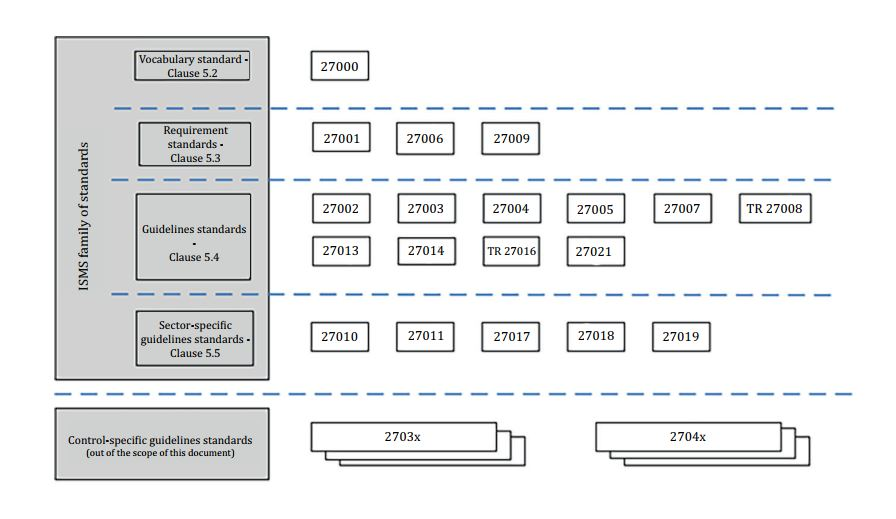
\includegraphics[scale=0.55]{fig/ISO27000.JPG}
    \caption{Família ISO 27000}
    \label{fig:testeISO}
\end{figure}


Conforme ilustrado na Figura~\ref{fig:testeISO}, a família ISO 27000 é organizada entre vocabulário, requisitos, guias e guias específicos.  


\item{Padrão que descreve uma visão geral e terminologia, conforme Figura 2.1:}

\begin{itemize}
    \item ISO/IEC 27000: Mostra uma visão geral da família ISO 27000 além de descrever conceitos básicos como vocabulário, termos e definições.
    \end{itemize}
    
    \item{Padrões que especificam requisitos de segurança, conforme Figura 2.1:}
    
    \begin{itemize}
    \item ISO/IEC 27001: Descreve os requisitos para estabelecer, implementar, operar, monitorar, revisar, manter e melhorar  sistemas de gestão da segurança da informação. 
    \item ISO/IEC 27006 Especifica requisitos para organismos que fornecem auditoria e certificação de sistemas de gestão de segurança da informação. 
    \item ISO/IEC 27009: Define os requisitos para o uso da ISO / IEC 27001 em qualquer setor específico(campo, área de aplicação ou setor de mercado).
    \end{itemize}
    
    \item{Padrões que descrevem diretrizes gerais, conforme Figura 2.1:}
    
    \begin{itemize}
    \item ISO/IEC 27002: Apresenta as melhores práticas que já foram testadas na prática e podem ser adaptadas aos requisitos individuais de cada empresa.
    \item ISO/IEC 27003: Guia de implementação do sistema de gestão de segurança da informação na ISO/IEC 27001.
    \item ISO/IEC 27004: Guia para auxiliar organizações a avaliar a performance da segurança da informação e efetividade do SGSI, para que se esteja de acordo com a  ISO/IEC 27001.
    \item ISO/IEC 27005: Guia para gestão de risco da segurança da informação.
    \item ISO/IEC 27007: Diretrizes para auditoria de sistemas de gestão da segurança da informação.
    \item ISO/IEC TR 27008: Diretrizes para os auditores sobre os controles de segurança da informação. 
    \item ISO/IEC 27013: Guia de orientação sobre a aplicação integrada da ISO / IEC 27001 e ISO / IEC 20000-1. 
    \item ISO/IEC 27014: Guia de princípios e processos para a governança da segurança da informação.
    \item ISO/IEC TR 27016: Gestão de segurança da informação - Economia organizacional
    \item ISO/IEC  27021: Especifica as competências e requisitos necessários para profissionais que atuam com um SGSI.
    \end{itemize}
   \
 \item{Normas que descrevem diretrizes específicas do setor, conforme Figura 2.1:}
 
 \begin{itemize}   
    \item ISO/IEC  27010: Guia da gestão de segurança da informação para as comunicações inter-setoriais e inter-organizacionais
    \item ISO/IEC  27011: Diretrizes de gestão da segurança da informação  para as organizações de telecomunicações com base na norma ISO/IEC 27002. 
    \item ISO/IEC  27017: Diretrizes para controles de segurança da informação aplicáveis ao fornecimento e uso de serviços em nuvem.
    \item ISO/IEC  27018: Código de práticas para proteção de informações de identificação pessoal (PII) em nuvens públicas atuando no processamento de PII.
    \item ISO/IEC T27019: Mostra controles específicos para a indústria de energia.
    
\end{itemize}

Juntos com os demais padrões da família ISO 27000 esses padrões formam um \textit{framework} criado para operar um sistema de gerenciamento da segurança da informação, com base em longas experiências de desenvolvimento \cite{disterer2013}. O foco principal desse TCC é nas ISOs 27001 e 27002 que definem processos para seleção e implantação de controles que ajudam a reduzir os riscos de possíveis vulnerabilidades.


\subsection{ISO 27001}

A norma ISO/IEC 27001 é um padrão internacional que define os requisitos necessários para estabelecer, implementar, manter e melhorar continuamente um SGSI. A norma também inclui requisitos para a avaliação e tratamento de riscos da segurança da informação para a necessidade de cada organização. Os requisitos definidos na norma são genéricos, permitindo que organizações de diferentes tamanhos possam aplicá-los. É importante ressaltar que todos requisitos da seção 4 até o 10 são obrigatórios para que uma organização esteja em conformidade coma a norma. Os controles do "anexo A" {} presentes na ISO/IEC 27001 devem ser implementados se estiverem presentes na declaração de aplicabilidade, juntamente com uma justificativa para inclusão \cite{ISOPDF}. 

A norma ISO/IEC 27001 \cite{ISOPDF} é estruturada da seguinte maneira:

\begin{itemize}
\item Seção 0: Introdução

    Descreve o objetivo da norma e sua importância de integração nos processos da própria organização além de mostrar sua compatibilidade com outras normas de sistemas de gestão.
\item Seção 1: Escopo

    Mostra a abrangência da norma explicando que seus requisitos são genéricos e  que são aplicáveis em qualquer organização, independente do tipo tamanho ou natureza.
\item Seção 2: Referência normativa

    Explica que indispensável a utilização da norma ISO/IEC 27000  como referência para do documento em questão.
\item Seção 3: Termos e definições

    Explica que os termos e definições presentes na ISO/IEC 27000 serão utilizados no documento.
\item Seção 4: Contexto da organização

    A sessão explica que a organização deve determinar questões internas e externas, definir as partes interessadas e seus requisitos, além de definir um escopo da aplicabilidade do SGSI.
\item Seção 5: Liderança

    A sessão explica que a alta direção deve demonstrar sua liderança e comprometimento, estabelecer uma política de segurança de informação  e assegurar que as responsabilidades e autoridades dos papéis relevantes para a segurança da informação sejam atribuídos e comunicados.
\item Seção 6: Planejamento
    Explica que a organização deve determinar riscos e oportunidades que precisam ser consideradas , aplicar um processo de avaliação e tratamento de riscos e definir objetivos da segurança da informação. 
\item Seção 7: Apoio 

    Explica que a organização deve prover recursos necessários para um SGSI, além de determinar competências, conscientizar colaboradores, prover comunicação interna e externa relevantes além de documentar informações.  

\item Seção 8: Operação

    Explica que a organização deve planejar, implementar e controlar processos, para atender os requisitos de um SGSI, além de avaliar e tratar os riscos de segurança da informação.

\item Seção 9: Avaliação do desempenho

    Explica que a organização deve monitorar, medir analisar e avaliar um SGSI, além de realizar auditorias internas. Também é definido uma análise critica pela direção sobre o SGSI para  para assegurar a sua contínua adequação, pertinência e eficácia. 

\item Seção 10: Melhoria
   
    Essa seção explica sobre não conformidades, ação corretiva e melhoria contínua do sistema de gestão
da segurança da informação.

\item Anexo A
   
    Referência aos controles e objetivos de controles presentes na ISO/IEC 27002

 \end{itemize}

%https://advisera.com/27001academy/pt-br/o-que-e-a-iso-27001/

\subsection{ISO 27002}

A norma ISO/IEC 27002 é projetada para ser utilizada como referência na implantação de um SGSI, referente a ISO/IEC 27001 ou como orientação para se implementar controles de segurança baseados em boas práticas. A ISO/IEC 27002 é dividida em 14 seções de controles da segurança da informação, 35 objetivos de controles e 114 controles. A ordem como se encontram as seções não define o grau de importância para cada uma, isso é definido por cada organização que deve identificar a sua aplicabilidade nos processos do negócio \cite{ISO27002}.

%Cada seção de controle da segurança da informação possui um ou mais objetivos de controles. 

A seleção de quais controles da segurança da informação serão usados depende das decisões da organização, baseadas nos critérios para aceitação de risco, nas opções para tratamento do risco e no enfoque geral da gestão de risco presente na organização. Também é importante ressaltar a importância dos controles estarem de acordo com as legislações e regulamentações nacionais e internacionais. A norma em questão é um ponto de partida para o desenvolvimento de diretrizes próprias para a organização. É importante frisar que nem todos os controles e diretrizes presentes na norma podem ser aplicados, pois os mesmos podem não ser relevantes ou suficientes dependendo da análise de risco presente nos requisitos da segurança de informação \cite{ISO27002} .

As seções principais possuem um objetivo de controle, que define o que se espera ser alcançado e um ou mais controles que podem ser usados para se alcançar o seu objetivo de controle. Os controles definem as medidas e ações que devem tomadas para atender ao objetivo de controle, cada controle possui uma diretriz para implementação com informações detalhadas que apoiam a execução do controle. Informações adicionais podem ser mostradas em alguns controles, para apresentar dados de questões legais e referências normativas. As seções, juntamente com seus objetivos, são como segue \cite{ISO27002};

% AQUI SEÇÃO 5
\begin{itemize}
  \item \textbf{Seção 5: Políticas de segurança da informação}
  
    Possui um objetivo de controle: Orientação da direção para segurança da informação.
    
\textit{     \textbf{Orientação da direção para segurança da informação:} }
     
     Tem como objetivo prover orientação da direção e apoio para a segurança da informação de acordo com os requisitos do negócio e com as leis e regulamentações relevantes.
  \end{itemize}
% AQUI SEÇÃO 6
\begin{itemize}
    \item \textbf{Seção 6: Organização da segurança da informação} 
    
    Possui dois objetivos: dispor sobre a  organização interna e sobre os dispositivos móveis e trabalho remoto
    
   \textit{ \textbf{Organização interna:} }
    
    Tem como objetivo estabelecer uma estrutura de gerenciamento, para iniciar e controlar a implementação da segurança da informação dentro da organização.
    
  \textit{  \textbf{Dispositivos móveis e trabalho remoto:}}
    
    Tem como objetivo garantir a segurança das informações no trabalho remoto e no uso de dispositivos móveis.
    
\end{itemize}
% AQUI SEÇÃO 7
\begin{itemize}
    \item \textbf{Seção 7: Segurança em recursos humanos}
    
    Possui três objetivos de controle: Antes da contratação, Durante a contratação e Encerramento e mudança da contratação.
    
  \textit{\textbf{Antes da contratação:}}
    
    Tem como objetivo assegurar que funcionários e partes externas entendem as suas responsabilidades e estão em conformidade com os papéis para os quais eles foram selecionados.

  \textit{\textbf{Durante a contratação:}}
    
    Tem como objetivo assegurar que os funcionários e partes externas estão conscientes e cumprem as suas responsabilidades pela segurança da informação.

    \textit{\textbf{Encerramento e mudança da contratação:} }
    
    Tem como objetivo proteger os interesses da organização como parte do processo de mudança ou encerramento da contratação.
\end{itemize}
% AQUI SEÇÃO 8
\begin{itemize}
    \item \textbf{Seção 8 : Gestão de ativos} 
    
    Possui três objetivos de controle: Responsabilidade pelos ativos, Classificação da informação, Tratamento de mídias.
    
    \textit{\textbf{Responsabilidade pelos ativos:} }
    
    Tem como objetivo identificar os ativos da organização e definir as devidas responsabilidades pela proteção dos ativos.
    
    \textit{\textbf{Classificação da informação:}}
    
    Tem como objetivo assegurar que a informação receba um nível adequado de proteção, de acordo com a sua importância para a organização.
    
    \textit{\textbf{Tratamento de mídias:} }
    
    Tem como objetivo prevenir a divulgação não autorizada, modificação, remoção ou destruição da informação armazenada nas mídias.

\end{itemize}
% AQUI SEÇÃO 9
\begin{itemize}
    \item  \textbf{Seção 9: Controle de acesso}
    
    Possui três objetivos de controle: Requisitos do negócio para controle de acesso, Responsabilidades dos usuários e  Controle de acesso ao sistema e à aplicação.
    
    \textit{\textbf{Requisitos do negócio para controle de acesso:}}
    
    Tem como objetivo limitar o acesso à informação e aos recursos de processamento da informação.
    
  \textit{  \textbf{Gerenciamento de acesso do usuário:}}
    
    Tem como objetivo assegurar acesso de usuário autorizado e prevenir acesso não autorizado a sistemas e serviços.
    
    \textbf{Responsabilidades dos usuários:} 
   
    Tem como objetivo tornar os usuários responsáveis pela proteção das suas informações de autenticação.
    
    \textit{\textbf{Controle de acesso ao sistema e à aplicação:} }
    
    Tem como objetivo prevenir o acesso não autorizado aos sistemas e aplicações.
\end{itemize}
% AQUI SEÇÃO 10
\begin{itemize}
    \item \textbf{Seção 10: Criptografia}
    
    Possui um objetivo de controle: Controle de acesso ao sistema e à aplicação
    
    \textit{\textbf{Controles criptográficos: } }
    
    Tem como objetivo assegurar o uso efetivo e adequado da criptografia para proteger a confidencialidade, autenticidade e/ou a integridade da informação.
\end{itemize}
%------------- AQUI SEÇÃO 11-----------------
\begin{itemize}
    \item \textbf{Seção 11: Segurança física e do ambiente}
    
    Possui dois objetivos de controle: Áreas seguras e Equipamentos.
    
    \textit{\textbf{Áreas seguras:}}
    
    Tem como objetivo prevenir o acesso físico não autorizado, danos e interferências com os recursos de processamento das informações e as informações da organização. 
    
   \textit{ \textbf{Equipamentos:} }
    
    Tem como objetivo impedir perdas, danos, furto ou roubo, ou comprometimento de ativos e interrupção
das operações da organização.
\end{itemize}
% --------------AQUI SEÇÃO 12------------------
\begin{itemize}
    \item \textbf{Seção 12: Segurança nas operações}
    
    Possui sete objetivos de controle: Responsabilidades e procedimentos operacionais, Proteção contra malware, Cópias de segurança, Registros e monitoramento, Controle de software operacional, Gestão de vulnerabilidades técnicas e Considerações quanto à auditoria de sistemas de informação.
    
  \textit{  \textbf{Responsabilidades e procedimentos operacionais:}}
    
    Tem como objetivo Garantir a operação segura e correta dos recursos de processamento da informação.
    
  \textit{  \textbf{Proteção contra malware:}}
    
    Tem como objetivo assegurar que as informações e os recursos de processamento da informação
estão protegidos contra malware.
    
   \textit{ \textbf{Cópias de segurança:}}
    
    Tem como objetivo proteção contra perda de dados.
    
   \textit{ \textbf{Registros e monitoramento:}}
    
    Tem como objetivo registrar eventos e gerar evidências.
    
    \textit{\textbf{Controle de software operacional:}}
    
    Tem como objetivo assegurar a integridade dos sistemas operacionais.
    
    \textit{\textbf{Gestão de vulnerabilidades técnicas:}}
    
    Tem como objetivo prevenir a exploração de vulnerabilidades técnicas.
    
  \textit{  \textbf{Considerações quanto à auditoria de sistemas de informação:}}

     Tem como objetivo Minimizar o impacto das atividades de auditoria nos sistemas operacionais.
\end{itemize}
% --------------AQUI SEÇÃO 13------------------
\begin{itemize}
    \item \textbf{Seção 13: Segurança nas comunicações }
    
    Possui dois objetivos de controle: Gerenciamento da segurança em redes e Transferência de informação.
    
    \textit{ \textbf{Gerenciamento da segurança em redes}}
    
     Tem como objetivo Assegurar a proteção das informações em redes e dos recursos de processamento da informação que os apoiam.

    \textit{ \textbf{Transferência de informação}}
    
     Tem como objetivo Manter a segurança da informação transferida dentro da organização e com
quaisquer entidades externas.
    
\end{itemize}
% --------------AQUI SEÇÃO 14------------------
\begin{itemize}
    \item \textbf{Seção 14: Aquisição, desenvolvimento e manutenção de sistemas}
    
    Possui três objetivos de controle: Requisitos de segurança de sistemas de informação, Segurança em processos de desenvolvimento e de suporte e Dados para teste.
    
    \textit{\textbf{Requisitos de segurança de sistemas de informação}}
    
    Tem como objetivo garantir que a segurança da informação é parte integrante de todo o ciclo de vida dos sistemas de informação. Isto também inclui os requisitos para sistemas de informação que fornecem serviços sobre as redes públicas.
    
   \textit{ \textbf{Segurança em processos de desenvolvimento e de suporte}}
    
    Tem como objetivo garantir que a segurança da informação está projetada e implementada no ciclo de vida de desenvolvimento dos sistemas de informação.
    
  \textit{  \textbf{Dados para teste}}\textit{}
    
    Tem como objetivo assegurar a proteção dos dados usados para teste.
\end{itemize}
% --------------AQUI SEÇÃO 15------------------
\begin{itemize}
    \item \textbf{Seção 15: Relacionamento na cadeia de suprimento}
    
    Possui dois objetivos de controle: Segurança da informação na cadeia de suprimento, Gerenciamento da entrega do serviço do fornecedor.
    
   \textit{ \textbf{Segurança da informação na cadeia de suprimento}}
    
    Tem como objetivo garantir a proteção dos ativos da organização que são acessíveis pelos fornecedores.
    
   \textit{ \textbf{Gerenciamento da entrega do serviço do fornecedor}}
    
    Tem como objetivo Manter um nível acordado de segurança da informação e de entrega de serviços em consonância com os acordos com fornecedores.
\end{itemize}
% --------------AQUI SEÇÃO 16------------------
\begin{itemize}
    \item \textbf{Seção 16: Gestão de incidentes de segurança da informação}
    
    Possui um objetivo de controle: Gestão de incidentes de segurança da informação e melhorias.
    
    \textit{\textbf{Gestão de incidentes de segurança da informação e melhorias}}
    
    Tem como objetivo assegurar um enfoque consistente e efetivo para gerenciar os incidentes de segurança da informação, incluindo a comunicação sobre fragilidades e eventos de segurança da informação.
\end{itemize}
% --------------AQUI SEÇÃO 17------------------
\begin{itemize}
    \item \textbf{Seção 17: Aspectos da segurança da informação na gestão da continuidade do negócio}
    
    Possui dois objetivos de controle: Continuidade da segurança da informação e Redundâncias.
    
    \textit{\textbf{Continuidade da segurança da informação}}
    
    Tem como objetivo a continuidade da segurança da informação deve ser contemplada nos sistemas de gestão da continuidade do negocio da organização.
    
    \textbf{Redundâncias}
    
     Tem como objetivo assegurar a disponibilidade dos recursos de processamento da informação.
\end{itemize}
% --------------AQUI SEÇÃO 18------------------
\begin{itemize}
    \item \textbf{Seção 18: Conformidade}
    
    Possui dois objetivos de controle: Conformidade com requisitos legais e contratuais e Análise crítica da segurança da informação
    
   \textit{ \textbf{Conformidade com requisitos legais e contratuais}}
    
    Tem como objetivo evitar violação de quaisquer obrigações legais, estatutárias, regulamentares ou contratuais relacionadas á segurança da informação e de quaisquer requisitos de segurança.
    
    \textit{\textbf{Análise crítica da segurança da informação}}
    
    Tem como objetivo garantir que a segurança da informação está implementada e operada de acordo com as politicas e procedimentos da organização.
\end{itemize}


\section{Segurança em Ecossistema de Software Móvel}

Bosch e Bosch-Sijtsema \cite{bosch2010integration} definem Ecossistema de Software como uma plataforma de software que consiste em um conjunto de desenvolvedores externos e internos juntamente com uma comunidade que compõem soluções  relevantes para satisfazer suas necessidades.

De acordo com Fontão e colegas \cite{fontao}, Ecossistema de Software móvel é um conjunto de sistemas colaborativos, usuários e desenvolvedores em uma relação de cooperação e competição. Um ECOSs Móvel possui todas as atribuições e conceitos de um ecossistema de software com diferença que ele é voltado para o contexto de dispositivos móveis, nesse caso \textit{smartphones} \cite{mestradoCaio}.

Para Furnell e colegas \cite{furnell2009integrated}, os principais elementos que desafiam a implantação de segurança de informação em organizações são os fatores humanos, organizacionais e tecnológicos. Alguns dos exemplos de fatores humanos são a falta de treinamento ou experiência, cultura da organização. Para fatores organizacionais foram encontrados desafios como estimativa de risco errada, falta de verba, baixa prioridade e distribuição equivocadas das responsabilidades de TI. Finalizando, os desafios tecnológicos são a complexidade do sistema, vulnerabilidades em sistemas e aplicações, falta de eficiência, ferramentas de segurança e mobilidade e distribuição de acesso.

Watanabe \cite{watanabe2017understanding} investigou a vulnerabilidade de aplicativos pagos e gratuitos, descobrindo que 70{\%} dos aplicativos gratuitos e 50{\%} dos aplicativos pagos eram vulneráveis devido a bibliotecas utilizadas no desenvolvimento. Descobriu-se também que aplicativos mais caros/populares tendem a ter mais vulnerabilidades e que aplicativos pagos tendem a não serem atualizados por períodos mais longos do que os aplicativos gratuitos, portanto as bibliotecas vulneráveis nos aplicativos pagos, não são atualizadas por períodos mais longos do que os aplicativos gratuitos.  O ultimo achado identificou que aproximadamente metade das vulnerabilidades detectadas pelas ferramentas de verificação de vulnerabilidade existentes são encontradas em código inacessível.

%rever
Segundo Jaramillo \cite{jaramillo2013cross}, dispositivos \textit{mobile} são criados para serem usados em diversos locais, isso tende a expor o dispositivo a mais riscos de segurança.  Para isso, organizações que usam dispositivos \textit{mobile} em seus serviços devem considerar os seguintes fatores de segurança:
\begin{itemize}
    \item \textbf{Segurança Física:} Quem tem a posse do aparelho, se ele é compartilhado com mais usuários e se o dispositivo já foi roubado ou perdido.
    \item \textbf{Segurança de Acesso:} Que controles garantem que o usuário atual tem acesso a dados e programas do dispositivo.   
    \item \textbf{Segurança de Dados:} Como os dados são protegidos no aparelho. 
    \item \textbf{Segurança de Redes:} Aparelhos \textit{mobile} são expostos a uma grande quantidade redes, que vão desde redes seguras até redes sem segurança alguma. Por essa razão segurança de redes é um ponto muito relevante na criação de um sistema.
    \item \textbf{Uso de Padrões:} Quando o usuário utiliza seu dispositivo tanto para tarefas pessoais ou de trabalho, a organização não consegue controlar ou  pré a provar a instalação de aplicativos que estão ao lado de aplicações disponibilizadas pela organização. 
    \item \textbf{Identidade:} Como assegurar a identidade do usuário e não somente a a do dispositivo rever tradução
\end{itemize}

A grande popularidade faz o sistema operacional Android ser o primeiro alvo de ataques de \textit{malware}. Um dos mecanismos usados pelo sistema para tentar evitar aplicativos maliciosos é o mecanismo de solicitação de permissão, prevenindo acessos em lista de contatos, mensagens de SMS e \textit{e-mails}. Entretanto muitos usuários ignoram os avisos de autorização por considerarem entediante e complicado. Com isso se faz necessário melhorar a efetividade do sistema de permissão, fazendo com que o usuário tenha fácil entendimento dos riscos. \cite{wang2017android}

%Para Fahl \cite{fahl2014hey} a evolução e ascensão das plataformas mobile tem contribuído para o crescimento de lojas de aplicativos (e.g google play, Apple store). Graças a posição de confiança no ecossistema de software, entretanto as mesmas lojas se invadidas representam uma ameaça ao usuário.

%\section{Mapeamento da literatura do uso da família 27000  em ecossistema de software móvel}

\chapter{\label{chap:intro}problemática e objetivo de pesquisa}


\section{Problema}

A segurança tem se tornado uma preocupação grande entre os usuários de dispositivos \textit{mobile} (ou móvel), porém essa preocupação varia de acordo com o sistema operacional utilizado pelo usuário. De acordo com o estudo de Reinfelder e colegas \cite{reinfelder2014differences}, usuários de Android são mais cientes a respeito de segurança e  privacidade, pois questões e permissões de privacidade são importantes para eles na decisão de instalar um novo aplicativo . A conclusão provisória mostrou que usuários de Android parecem ter mais consciência da privacidade do que os usuários do iOS, entretanto é necessária uma investigação mais aprofundada.

%imagem aqui

Alguns autores possuem resultados em comum a respeito das dificuldades da adoção de segurança de informação em organizações. Jaramilo e colegas \cite{jaramillo2013cross} comenta sobre a diferença de prioridades institucionais. Furnell e colegas \cite{furnell2009integrated} dividiram as categorias em fator humano, técnico e institucional. Disterer \cite{disterer2013} afirma que a segurança da informação deve ser organizacionalmente estabelecida na organização, para que medidas possam ser promovidas e estabelecidas para todos.


Castle e colegas \cite{castle2016let} avaliaram os desafios de segurança em serviços financeiros digitais em dispositivos móvel e verificou que os desenvolvedores entrevistados se preocupam com questões de segurança. Com isso o autor levantou a seguinte questão: \textit{“Quando desenvolvedores ou designers de produto querem aprender mais sobre opções de padrões para medidas de segurança, quais recursos eles devem usar?“}. O autor sugere o \textit{Stack Overflow} como fonte inicial de aprendizado, porém relata que a plataforma ainda oferece pouca consistência e padronização para boas práticas.

%ver como citar corretamente erdem do BIB
No estudo realizado por Steglich e colegas  \cite{caio2019} foi investigada a literatura no tópico de segurança da informação em organizações, com o foco na ISO 27000, mais especificamente na ISO 27001 e seus controles. Foi descoberto que apenas 34 dos 114 controles descritos na ISO 27001 estavam presentes na literatura de ecossistemas de software \textit{mobile} e apenas duas das quatorze seções tinham todo os seus controles representados na literatura, que eram as seções de políticas de segurança da informação e criptografia.  

Assim, no contexto de ecossistemas de software móvel, este TCC  buscou identificar se desenvolvedores externos ou internos adotam controles da ISO 27002 para o desenvolvimento de software \textit{mobile}.
\todo[inline]{tirei a parte do guia aqui, esta ok?}



\section{Objetivo geral}

O principal objetivo deste TCC é identificar por meio de uma \textit{survey} quais são os controles da ISO 27002 adotados no desenvolvimento de software móvel. Com o resultado desta \textit{survey} realizou-se uma análise dos resultados para entender qual eram as questões que os desenvolvedores levavam em consideração e quais eles não levavam no momento de desenvolver aplicações móveis.

 
\subsubsection{\textbf{Objetivos específicos:}}

Para atingir o objetivo geral deste trabalho de conclusão, definiu-se os seguintes objetivos específicos:

\begin{enumerate}
    \item Aprofundar o conhecimento sobre a literatura em segurança de informação baseado na ISO 27002 em ecossistemas de software \textit{mobile}.
    
    \item Definir e conduzir uma \textit{survey} baseado na revisão da literatura anterior de Steglich e colegas \cite{caio2019}.
    
    \item Analisar os resultados da \textit{survey} com o objetivo de compreender a preocupação dos desenvolvedores com as questões.
    
    
\end{enumerate}
%Quais são? teria que abrir o objetivo geral?


      

%\section{Cronograma}

%O cronograma foi dividido entre os 2 semestres do ano de 2020, contemplando a metodologia \textit{survey}. No primeiro semestre será elaborada uma análise critica da ISO 27000 separando as seções que sejam relevantes para o objetivo trabalho. No segundo semestre as seções serão validadas com especialistas para elaborar a \textit{survey} que irá gerar resultados  para elaborar um site com recomendações de boas práticas.

%\begin{figure}
%    \centering
%   \includegraphics[scale=0.59]{fig/crongrama.JPG}
%  \caption{Cronograma}
%   \label{fig:my_label}
%\end{figure}





%----------------------------------------------------------------------------------
% Exemplo do ambiente para citações diretas com mais de 3 linhas.
%
% Para citações diretas de até 3 linhas, faça assim:
% De acordo com Direto~(2011, p.~21): "bla bla bla, bla 'bla'."
\chapter{\label{chap:intro}Metodologia de Pesquisa}


A metodologia de pesquisa escolhida para este trabalho, é composta do entendimento e análise de uma revisão de literatura apresentada anteriormente por Steglich e colegas \cite{caio2019} e de uma \textit{survey} realizada com desenvolvedores de ECOSM. Para Kitchenham end Pfleeger \cite{pfleeger2001principles} uma \textit{survey} consiste em sistema de coleta de dados e informações objetivando decifrar conhecimentos e práticas adotadas pelos sujeitos da pesquisa.
   
As etapas que compõe uma pesquisa \textit{survey} são:  definição do objetivo da pesquisa, definição da população e da amostra, elaboração do questionário, coleta de dados, processamento dos dados, análise dos dados e divulgação dos resultados \cite{vieira2010dicionario}.

\begin{figure}
    \centering
    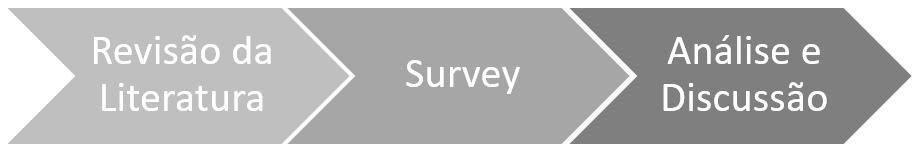
\includegraphics[scale=0.66]{fig/metodologia.PNG}
    \caption{Metodologia de Pesquisa}
    \label{fig:my_label}
\end{figure}


\section{\textbf{Revisão da Literatura e Definição do Escopo}}

%Pretendeu-se aprofundar o conhecimento na literatura de segurança em Ecossistemas de Software Móvel(ECOSM) e também em controles presentes na ISO 27002 utilizando como base a revisão da literatura feita por Steglich e colegas \cite{caio2019} que teve como objetivo identificar quais controles da ISO 27001 estão presentes na literatura de ECOSM, buscando verificar evidências sobre como eles são usados e o que a literatura relata sobre esses controles. O resultado do estudo mostrou que apenas 34 dos 114 controles da ISO 27001 estavam presentes na literatura de ECOSM e que apenas 2 de um total de 14 seções tinham seus respectivos controles evidenciados na literatura de ECOSM . Essas seções são, políticas de segurança da informação e criptografia. A falta de literatura sobre a maioria dos controles da ISO 27002, motivou o desenvolvimento deste trabalho.

 Com o objetivo de entender a  ISO 27002 e identificar quais os controles dela estão presentes na literatura,
 utilizou-se a revisão da literatura de Steglich e colegas \cite{caio2019}. Restringiu-se a literatura ao artigo citado, dado que o mesmo consolida toda  a literatura na área. O artigo é uma revisão de autoria do orientador desde TCC, realizada em 2019, quando este trabalho se iniciou. Este artigo teve como objetivo identificar quais controles da ISO 27001 estão presentes na literatura de ECOSM, buscando verificar evidências sobre como eles são usados e o que a literatura relata sobre esses controles. O resultado do estudo mostrou que apenas 34 dos 114 controles da ISO 27001 estavam presentes na literatura de ECOSM e que apenas 2 de um total de 14 seções tinham seus respectivos controles evidenciados na literatura de ECOSM . Essas seções são, políticas de segurança da informação e criptografia. A falta de literatura sobre a maioria dos controles da ISO 27002, motivou o desenvolvimento deste trabalho, que ocorreu da seguinte forma:
 
 \begin{itemize}
    \item Passo 1: Primeiramente realizou-se um estudo em profundidade com o objetivo de entender a ISO 27002 e seus controles.
   
    \item Passo 2: Identificação de quais seções presentes na ISO 27002 estava de acordo com proposta deste TCC.
    
     \item Passo 3: Reuniões para a decisão e deliberação de quais seções seriam mantidas e retiradas por estarem fora do escopo do trabalho.
      
    \item Passo 4: Revisão com um especialista, das seções da ISO 27002 que foram selecionadas.
  \end{itemize}

 
 %A partir da identificação de quais seções da ISO 27002 estavam de acordo com a proposta, e do estudo...
 \noindent \paragraph{\textbf{Passo 1:} A partir do estudo de Steglich e colegas \cite{caio2019} e do estudo aprofundado de quais seções da ISO 27002 estavam de acordo com a proposta, foi possível aprofundar o conhecimento sobre as normas e sua relevância para este trabalho.}
 
 \noindent \paragraph{\textbf{Passo 2:} Inicialmente começou-se interpretando as seções e seus controles verificando a complexidade de cada uma no contexto de ecossistema de software móvel. Na primeira seleção das seção alguns controles e objetivos de controle foram retirados por não estarem relacionados com desenvolvimento de de software.}
 
 \noindent 
    \paragraph{
    \textbf{Passo 3:} Para aprimorar a filtragem realizada inicialmente, foram realizadas discussões com 3 pesquisadores, com experiência nas áreas de auditoria, metodologia de pesquisa e ecossistemas de software móvel. Foram feitas reuniões de uma hora, conduzidas pelo autor deste trabalho e com isso foi possível eliminar as seções irrelevantes e manter outras.
    }
 
    \paragraph{
  A partir da filtragem de seções e controles com os pesquisadores, foi possível eliminar as Seções 5, 6, 7, 8, 11, 13, 15, 16, 17, 18 pois seus controles e objetivos de controle não se enquadravam no objetivo deste TCC, que  pretende ter como foco controles que se enquadrem no desenvolvimento de software mobile. Por exemplo, a Seção 7 trata Segurança dos Recursos Humanos. No entendimento do autor deste TCC e em alinhamento com os três pesquisadores que participaram das discussões nessa etapa inicial, entendeu-se que a Seção está fora do escopo de desenvolvimento de software, pois trata de como evitar o vazamento de informações por colaboradores. Detalhes podem ser consultados no apêndice B. As Seções 9, 10, 12, 14 foram mantidas e alguns de seus objetivos de controle retirados devido a análise conjunta dos pesquisadores durante a discussão. Após a filtragem das seções com os 3 pesquisadores, convidamos um especialista convidamos um especialista, com o intuito de validar o escopo das seções e das peguntas elaboradas. 
    }
    
  \noindent
    \paragraph{
    \textbf{Passo 4:} Visando confirmar a relevância dos controles selecionados, presentes na ISO/IEC 27002, buscou-se estratégias para que de fato os controles selecionados fossem relevantes para a execução de uma \textit{survey} com desenvolvedores de software móveis. Para isso, usou-se a abordagem de Entrevista com Especialistas para avaliação dos controles selecionados previamente, conforme recomendado por Flick \cite{flick2018introduction}. O autor esclarece que entrevistar especialistas pode servir a três propósitos: i) para exploração, para orientação em um novo campo, a fim de auxiliar a geração de hipóteses; ii) pode ser usada para coletar informações de contexto complementando percepções provenientes da aplicação de outros métodos; ou iii) pode também ser usada para geração de teorias que visam desenvolver uma tipologia ou uma teoria sobre uma questão a partir da reconstrução do conhecimento de vários especialistas. Com base no que foi expressado pelo autor \cite{flick2018introduction}, as entrevistas com os especialistas sarão utilizadas com o propósito ii), de coletar informações com a finalidade de complementar as percepções a respeito dos controles presentes na ISO/IEC 27002 que foram selecionados previamente e revisar a sua relevância.
    }
    
    \paragraph{
    Foi convidado, por conveniência, um especialista para participar desta avaliação, após a filtragem com os três pesquisadores para selecionar os controles presentes na ISO/IEC 27002, que fossem direcionados para a área da computação e elaborar perguntas referentes a cada controle da ISO/IEC 27002. Para que as perguntas sejam utilizadas na elaboração de um questionário com diversos desenvolvedores. O perfil deste especialista é como segue:}   
    
    \paragraph{
    O entrevistado é de Alvorada, RS, cidade da região metropolitana de Porto Alegre, já tendo atuado em outros países em projetos de tecnologias móveis, sendo desenvolvedor da área há 12 anos e atualmente como instrutor. Ao longo destes 12 anos, este especialista colaborou com os ECOS Android, iOS, WindowsPhone e Blackberry.
    }
    
    \paragraph{
    A partir da entrevista com o especialista foi possível verificar se as perguntas condiziam com preocupações ou atividades de um desenvolvedor de aplicações móveis. Nesta revisão ficou resolvido que o a maioria das perguntas estavam adequadas com o tema proposto e foram sugeridas as remoções de 21 perguntas de um total de 78.}
    
    %\todo[inline]{ Posteriormente a entrevista com o especialista, 3 pesquisadores da área de ES reconheceram outro conjunto de perguntas que poderiam ser removidas, pois condiziam com elementos de gestão organizacional e não de TI ou desenvolvimento de software.(ESSA PARTE ESTÁ ADEQUADA?)}
    
 

 
 

 

 
 %Nas figuras 5.1, 5.2, 5.3 e 5.4 estão representados os controles mantidos \todo[inline]{citar apendice ? e onde fica melhor de colocar essa frase? "nas figuras..."}
 
 %e serão validadas futuramente com um especialista numa entrevista, para que assim seja possível elaborar a survey e dar continuidade as etapas da metodologia de pesquisa do trabalho.  
 
 
 
 






\section{\textbf{\textit{Survey}}} Definiu-se como objetivo de pesquisa, conhecer quais os controles da ISO 27002 são adotados ou não por desenvolvedores de software móvel. Para atingir o objetivo do trabalho os seguintes passos, com base no artigo de Kitchenham end Pfleeger \cite{pfleeger2001principles} foram realizados:
\begin{itemize}

\item \textbf{Construir instrumento de coleta:} Para elaborar o questionário serão considerados os resultados anteriores das entrevistas com especialistas. O perfil desejado para a realização da pesquisa será de desenvolvedores de software mobile.

\item \textbf{Validação do instrumento de coleta:} O instrumento foi validado com dois participantes. O primeiro participante é de Manaus, AM, sendo professor e pesquisador com 10 anos de experiência na área, sendo 2 anos como desenvolvedor de aplicações, 4 anos como evangelista de desenvolvedores e 4 anos como pesquisador da área. Já colaborou nos ECOS Android, Windows Phone, Nokia e Symbian. Com este participante foi possível  melhorar o entendimento de algumas perguntas, com o intuito de deixar-las mais claras, além de ter uma estimativa do tempo de 20 minutos de resposta do questionário. O segundo participante é professor no Instituto Federal do Rio Grande do Sul e tem 3 anos de pesquisa com empresas em desenvolvimento mobile. Com este participante foi possível avaliar o conteúdo técnico de algumas perguntas para que os futuros respondentes não tivessem dúvidas ao responder o questionário.


%O questionários será validado com desenvolvedores mobile com experiência alguns anos de experiência. Será realizado um piloto do questionário com colegas de curso que entendem de desenvolvimento mobile

 \textbf{Piloto:} Também como parte da validação do instrumento, realizou-se o piloto com o objetivo identificar qualquer prolema com o questionário, antes da coleta da coleta dos dados. Este piloto foi realizado com 2 participantes. 
 
 O primeiro participante é estudante de Engenharia de Software na Pontifícia Universidade Católica do Rio Grande do Sul e participou do programa de capacitação Apple Developer Academy. O participante levou  14 minutos para responder a \textit{survey} e considerou que o fluxo nas das questões estavam bem estruturadas, sem a necessidade de alguma alteração.
 
 O segundo participante é estudante de ciência da computação na PUCRS e trabalha como \textit{quality assurance}. O participante levou 16 minutos para responder a \textit{survey} e verificou alguns erros de formatação no texto, que foram corrigidos posteriormente.  
 

\item \textbf{Coleta dos Dados:} A coleta foi realizada somente de maneira online pelas limitações da pandemia. Inicialmente o instrumento foi divulgado no LinkedIn com o objetivo de atingir a rede de contatos que se enquadravam no perfil desejado de desenvolvedores mobile. O instrumento também foi divulgado em grupos de desenvolvedores iOS e Android no Slack e Facebook. A \textit{survey} conforme foi distribuída, pode ser consultada no Apêncide A.

Devido a baixa taxa de respondentes entrou-se em contato individualmente com desenvolvedores de dispositivos móveis presentes na rede de contatos do LinkedIn, com o objetivo de obter mais respostas. Os pesquisadores que auxiliaram na separação das seções da ISO 27002 também auxiliaram na divulgação da \textit{survey} , divulgando-a para sua rede de contatos. 


\item \textbf{Analisar resultados:} Com o resultado do questionário foi realizada a análise dos dados, que pode ser consultada no Capítulo 5. Separou-se cada questão individualmente, observando se o seu resultado demonstrava ou não uma preocupação dos desenvolvedores.
\end{itemize}

%\todo[inline]{Tiro tudo isso aqui, certo? virou projeto futuro} 
%\section{\textbf{Definição do Guia de Recomendações}}

%Requisitos de segurança como confidencialidade, integridade são abstratos e suas aplicações necessitam de uma orientação para serem seguidos, para que seja possível atender aos requisitos. Com os resultados da \textit{survey} ira ser criado um guia de recomendações de boas práticas com objetivo de auxiliar desenvolvedores a adotarem os controles previstos na ISO 27002. 

%No processo para a elaboração do guia de recomendações pretende-se desenvolver um critério para a categorização de cada uma das orientações. O principal objetivo por trás dessa classificação é preparar a base para expressar esses guias em uma linguagem formal e argumentar sobre sua satisfação \cite{zhioua2016security}.



 \chapter{\label{chap:intro}Análise Dos Resultados}
 




\section{Resultados da \textit{Survey}}

Após a conclusão do processo de coleta dados, com o objetivo de entender quais são as preocupações de desenvolvedores de software móveis no desenvolvimento de aplicações, destaca-se nessa seção o resultado obtido na survey. A survey teve um total de 20 respondentes.

O público que respondeu essa pesquisa tem em média 5 anos de experiência com desenvolvimento de aplicações  para dispositivos móveis e em sua maioria tem experiência com a plataforma Android. 

\begin{figure}
    \centering
    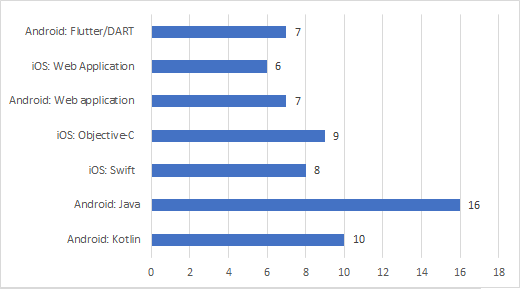
\includegraphics[scale=0.9]{fig/plataformas.PNG}
    \caption{Plataformas utilizadas pelos entrevistados}
    \label{fig:my_label}
\end{figure}



\begin{figure}[t]
\centering
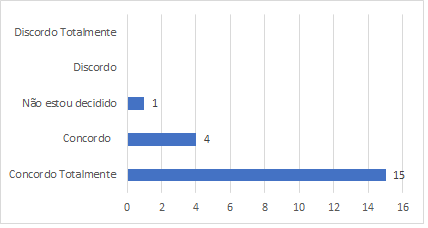
\includegraphics[scale=0.8]{figuras das questoes/1.1.PNG}
\caption{Preocupo-me com o controle de acesso de usuários nos sistemas que desenvolvo.}
\end{figure}


\begin{figure}[!t]
\centering
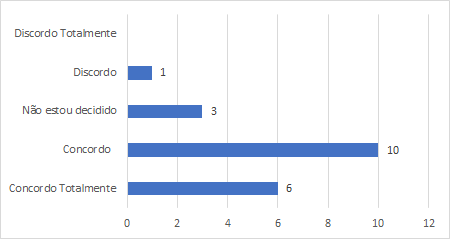
\includegraphics[scale=0.8]{figuras das questoes/1.2.PNG}
\caption{Preocupo-me em criar ou utilizar funcionalidades que permitam o bloqueio, remoção ou desabilitação rápida de usuários no sistema (por exemplo, funcionários que deixaram a empresa).}
\end{figure}

\begin{figure}[!t]
\centering
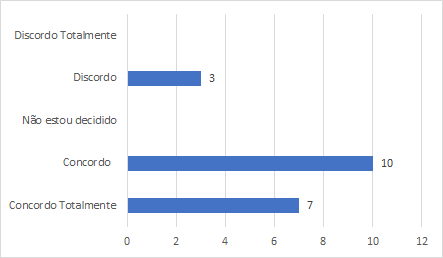
\includegraphics[scale=0.7]{figuras das questoes/1.3.png}
\caption{Preocupo-me em desenvolver funções que permitam a alteração de permissão no
sistema para todos os usuários, ou seja, que seja possível o gerenciamento de usuários.}
\end{figure}

\begin{figure}[!t]
\centering
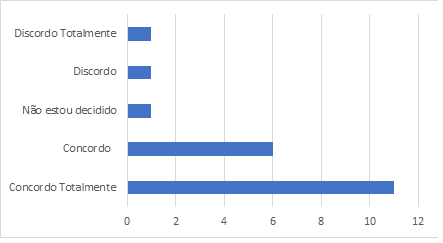
\includegraphics[scale=0.7]{figuras das questoes/1.4.png}
\caption{Preocupo-me em criar um registro central de direitos de acesso para cada usuário, ou seja, todos os usuários possuem um ID único.}
\end{figure}

\begin{figure}[!t]
\centering
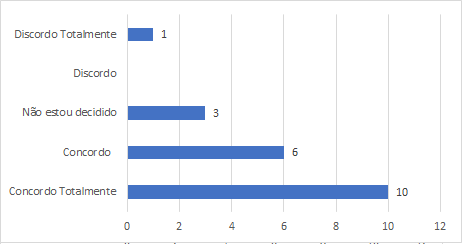
\includegraphics[scale=0.7]{figuras das questoes/2.1.png}
\caption{Preocupo-me em desenvolver funções que verifiquem a identidade de um usuário antes de fornecer uma informação de autenticação secreta, temporária, de substituição ou nova no sistema. (por exemplo e-mail de confirmação, SMS, aplicativos como Google autenticador).}
\end{figure}

\begin{figure}[!t]
\centering
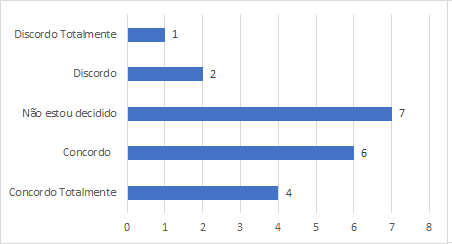
\includegraphics[scale=0.7]{figuras das questoes/2.2.png}
\caption{Preocupo-me em aprimorar o desenvolvimento de funcionalidades com autenticação secreta para acessos e logins. (autenticação por 2 fatores).}
\end{figure}

\begin{figure}[!t]
\centering
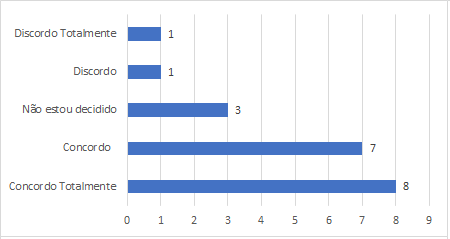
\includegraphics[scale=0.7]{figuras das questoes/2.3.png}
\caption{Preocupo-me para que a Informação de autenticação secreta temporária seja única para uma pessoa e que não possa ser facilmente adivinhada.}
\end{figure}

\begin{figure}[!t]
\centering
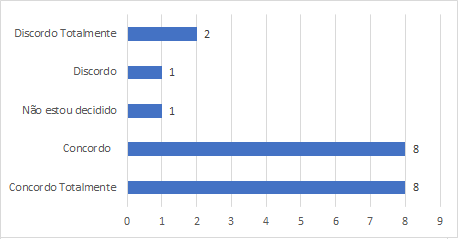
\includegraphics[scale=0.7]{figuras das questoes/2.4.png}
\caption{Preocupo-me em fornecer recursos para que o usuário consiga resguardar sua privacidade durante o processo de autenticação.}
\end{figure}

\begin{figure}[!t]
\centering
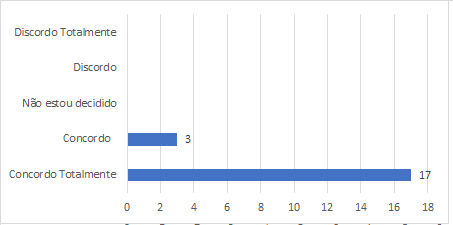
\includegraphics[scale=0.7]{figuras das questoes/2.5.png}
\caption{Preocupo-me em não mostrar dados sensíveis do usuário (status, informações pessoais, etc.) de aplicações até que o processo de Log-on tenha sido concluído com sucesso.}
\end{figure}

\begin{figure}[!t]
\centering
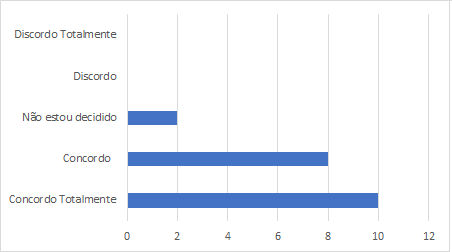
\includegraphics[scale=0.7]{figuras das questoes/2.6.png}
\caption{Preocupo-me em validar informações de entrada no sistema somente quando todos os dados de entrada estiverem completos.}
\end{figure}

\begin{figure}[!t]
\centering
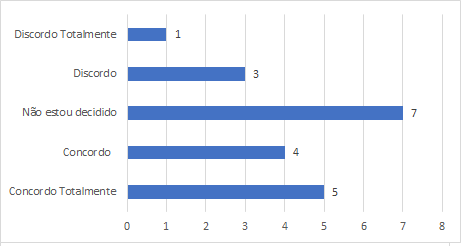
\includegraphics[scale=0.7]{figuras das questoes/2.7.png}
\caption{Caso ocorra um erro na validação das informações de entrada me preocupo em não identificar qual parte do dado de entrada está correto ou incorreto (Ex: “Sua senha está incorreta”).}
\end{figure}

\begin{figure}[!t]
\centering
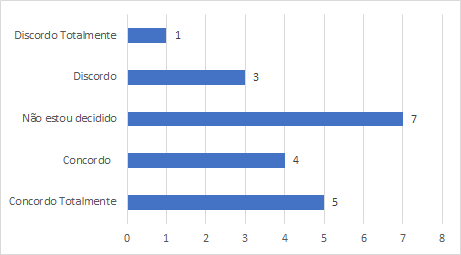
\includegraphics[scale=0.7]{figuras das questoes/2.8.png}
\caption{Preocupo-me em proteger o sistema contra tentativas consecutivas/repetidas de entrada forçada.}
\end{figure}

\begin{figure}[!t]
\centering
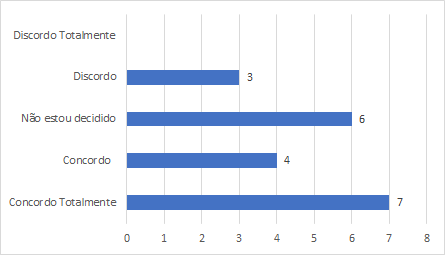
\includegraphics[scale=0.7]{figuras das questoes/2.9.png}
\caption{Preocupo-me em comunicar um evento de segurança caso uma tentativa potencial ou uma violação bem sucedida de entrada no sistema (log-on), seja detectada.}
\end{figure}

\begin{figure}[!t]
\centering
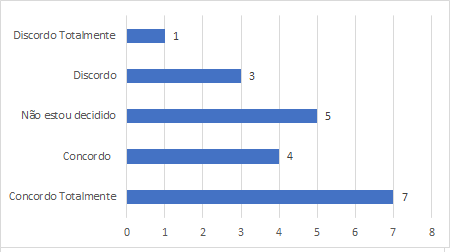
\includegraphics[scale=0.7]{figuras das questoes/2.10.png}
\caption{Preocupo-me em encerrar sessões inativas após um período de inatividade.}
\end{figure}

\begin{figure}[!t]
\centering
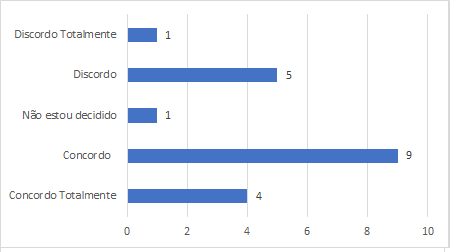
\includegraphics[scale=0.7]{figuras das questoes/2.11.png}
\caption{Preocupo-me em fazer sistemas que obriguem uma escolha de senha de qualidade, por exemplo, com no mínimo Oito Caracteres, misturar letras em caixa alta e baixa com números e caracteres não alfanuméricos).}
\end{figure}

\begin{figure}[!t]
\centering
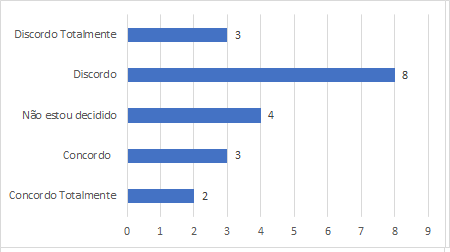
\includegraphics[scale=0.7]{figuras das questoes/2.12.png}
\caption{Preocupo-me em desenvolver sistemas que obriguem usuário a mudarem as suas senhas temporárias no primeiro acesso ao sistema (Sistema que coloca sua senha inicial como data de aniversário ou dígitos do RG).}
\end{figure}

\begin{figure}[!t]
\centering
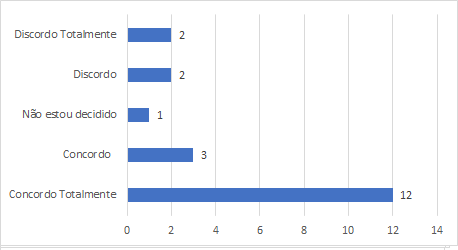
\includegraphics[scale=0.7]{figuras das questoes/2.13.png}
\caption{Preocupo-me em não permitir que a senhas possam ser mostradas na tela quando digitadas (Ex: Usar recurso do “olho” para revelar senha em um campo).}
\end{figure}

\begin{figure}[!t]
\centering
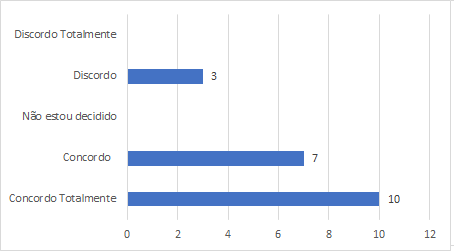
\includegraphics[scale=0.7]{figuras das questoes/3.1.png}
\caption{Preocupo-me com uso de criptografia para a proteção das informações sensíveis durante a comunicação em dispositivos móveis.}
\end{figure}

\begin{figure}[!t]
\centering
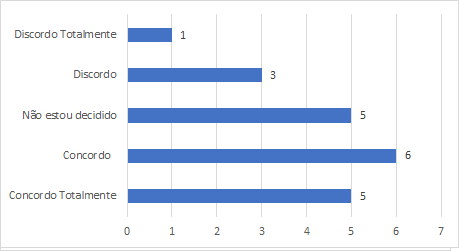
\includegraphics[scale=0.7]{figuras das questoes/3.2.png}
\caption{Preocupo-me em gerar chaves para diferentes sistemas criptográficos e diferentes aplicações.}
\end{figure}

\begin{figure}[!t]
\centering
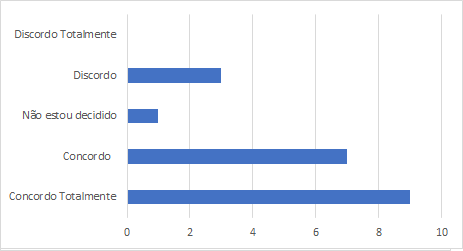
\includegraphics[scale=0.7]{figuras das questoes/4.1.png}
\caption{Preocupo-me com os impactos na segurança da informação quando ocorre alguma mudança no sistema.}
\end{figure}

\begin{figure}[!t]
\centering
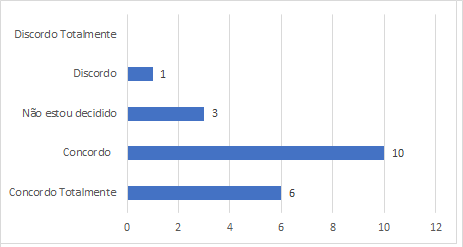
\includegraphics[scale=0.7]{figuras das questoes/4.2.png}
\caption{Preocupo-me em criar mecanismos para atender o crescimento da aplicação e possibilitar suportar demanda variável de acessos.}
\end{figure}

\begin{figure}[!t]
\centering
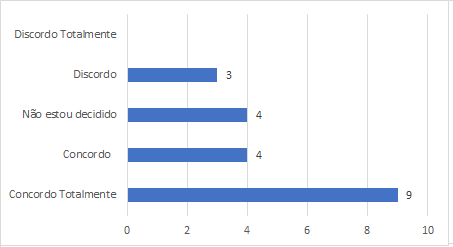
\includegraphics[scale=0.7]{figuras das questoes/4.3.png}
\caption{Preocupo-me para que dados sensíveis não sejam copiados para os ambientes de testes.}
\end{figure}

\begin{figure}[!t]
\centering
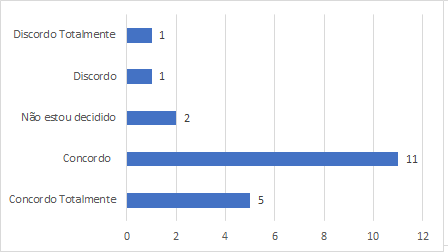
\includegraphics[scale=0.7]{figuras das questoes/5.1.png}
\caption{Preocupo-me em criar mecanismos para registrar os eventos do sistema.}
\end{figure}

\begin{figure}[!t]
\centering
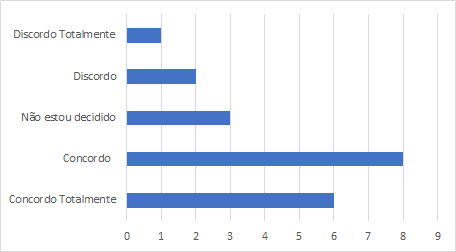
\includegraphics[scale=0.7]{figuras das questoes/5.2.png}
\caption{Preocupo-me com datas, horários e detalhes de eventos-chave, como, por exemplo, horário de entrada (log-on) e saída (log-off) no sistema.}
\end{figure}

\begin{figure}[!t]
\centering
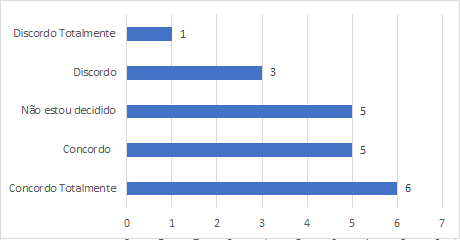
\includegraphics[scale=0.7]{figuras das questoes/5.3.png}
\caption{Preocupo-me com a identificação do dispositivo ou sua localização quando possível e o identificador do sistema.}
\end{figure}

\begin{figure}[!t]
\centering
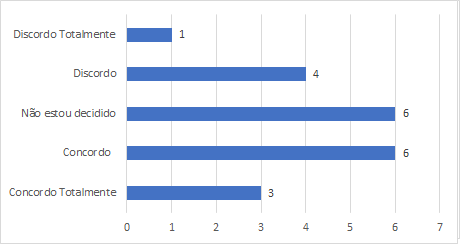
\includegraphics[scale=0.7]{figuras das questoes/5.4.png}
\caption{Preocupo-me com registro de tentativas de acesso ao sistema, aceitas e rejeitadas.}
\end{figure}
 
\begin{figure}[!t]
\centering
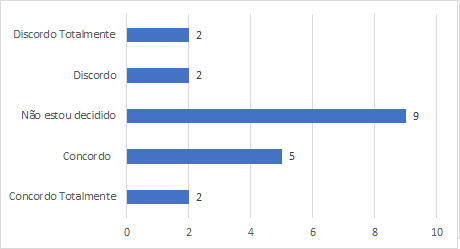
\includegraphics[scale=0.7]{figuras das questoes/5.5.png}
\caption{Preocupo-me com a coleta dos endereços e protocolos de rede no log.}
\end{figure}
 
\begin{figure}[!t]
\centering
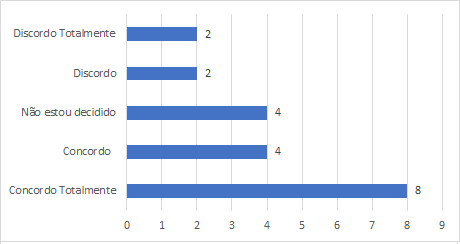
\includegraphics[scale=0.7]{figuras das questoes/5.6.png}
\caption{Preocupo-me para que arquivos de log não sejam editados ou excluídos sem a devida autorização.}
\end{figure}
   
\begin{figure}[!t]
\centering
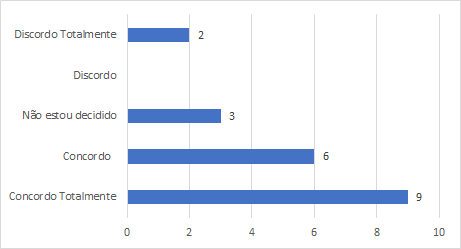
\includegraphics[scale=0.7]{figuras das questoes/6.1.png}
\caption{Preocupo-me em identificar falhas de segurança nas aplicações móveis que dou manutenção.}
\end{figure}

\begin{figure}[!t]
\centering
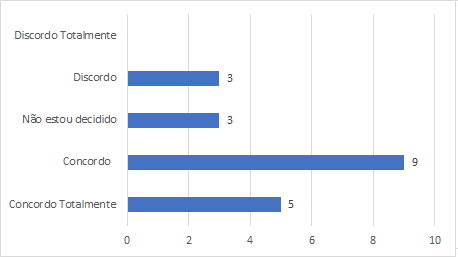
\includegraphics[scale=0.7]{figuras das questoes/6.2.png}
\caption{Respostas questão 6.2}
\end{figure}

\begin{figure}[!t]
\centering
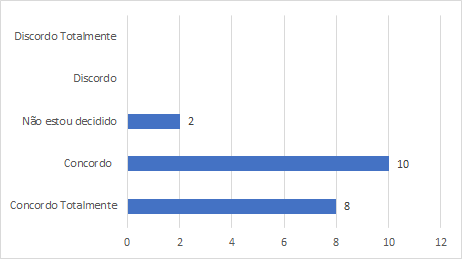
\includegraphics[scale=0.7]{figuras das questoes/6.3.png}
\caption{Respostas questão 6.3}
\end{figure}

\begin{figure}[!t]
\centering
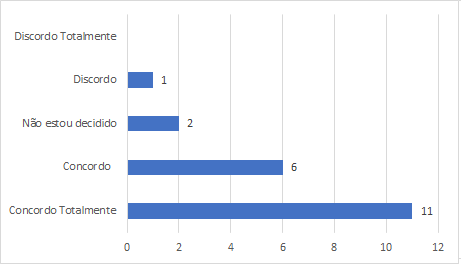
\includegraphics[scale=0.7]{figuras das questoes/6.4.png}
\caption{Respostas questão 6.4}
\end{figure}

\begin{figure}[!t]
\centering
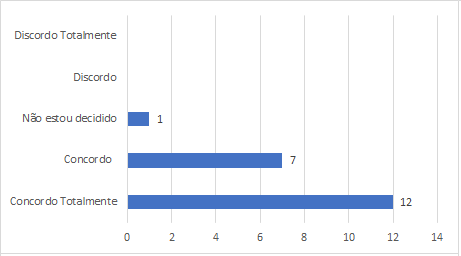
\includegraphics[scale=0.7]{figuras das questoes/6.5.png}
\caption{Respostas questão 6.5}
\end{figure}

\begin{figure}[!t]
\centering
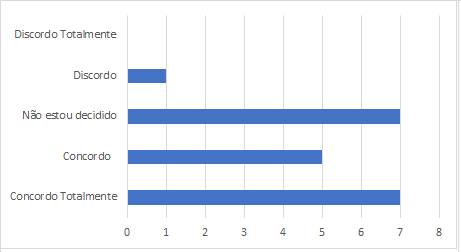
\includegraphics[scale=0.7]{figuras das questoes/6.6.png}
\caption{Respostas questão 6.6}
\end{figure}

\begin{figure}[!t]
\centering
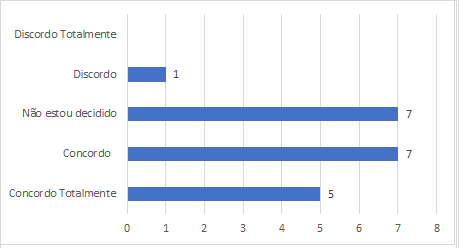
\includegraphics[scale=0.7]{figuras das questoes/6.7.png}
\caption{Respostas questão 6.7}
\end{figure}

\begin{figure}[!t]
\centering
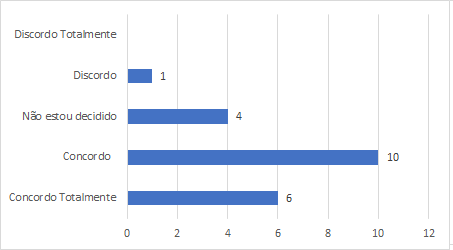
\includegraphics[scale=0.7]{figuras das questoes/6.8.png}
\caption{Respostas questão 6.8}
\end{figure}

\begin{figure}[!t]
\centering
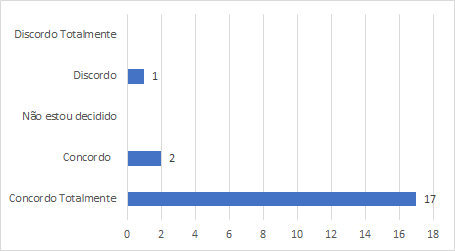
\includegraphics[scale=0.7]{figuras das questoes/6.9.png}
\caption{Respostas questão 6.9}
\end{figure}

\begin{figure}[!t]
\centering
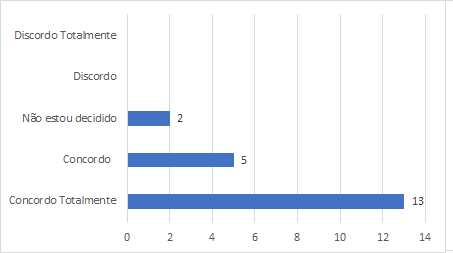
\includegraphics[scale=0.7]{figuras das questoes/6.10.png}
\caption{Respostas questão 6.11}
\end{figure}

\begin{figure}[!t]
\centering
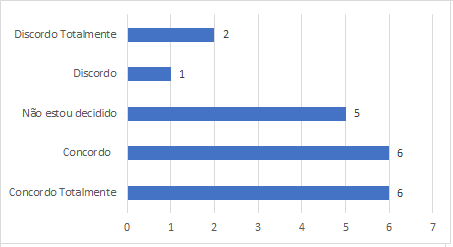
\includegraphics[scale=0.7]{figuras das questoes/6.11.png}
\caption{Respostas questão 6.11}
\end{figure}

\begin{figure}[!t]
\centering
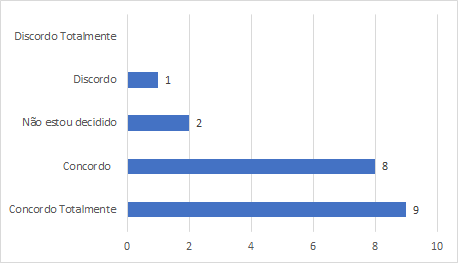
\includegraphics[scale=0.7]{figuras das questoes/6.12.png}
\caption{Respostas questão 6.12}
\end{figure}

\begin{figure}[!t]
\centering
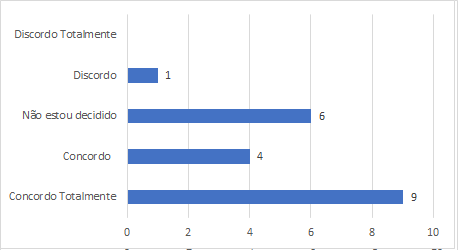
\includegraphics[scale=0.7]{figuras das questoes/6.13.png}
\caption{Respostas questão 6.13}
\end{figure}

\begin{figure}[!t]
\centering
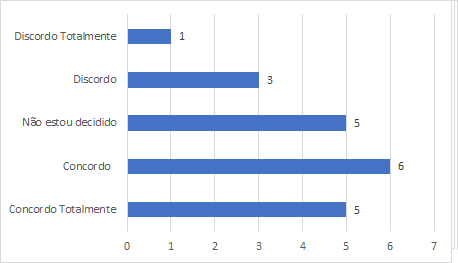
\includegraphics[scale=0.7]{figuras das questoes/6.14.png}
\caption{Respostas questão 6.14}
\end{figure}

\begin{figure}[!t]
\centering
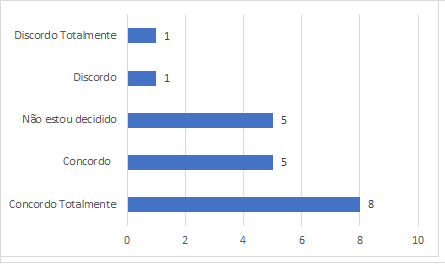
\includegraphics[scale=0.7]{figuras das questoes/6.15.png}
\caption{Respostas questão 6.15}
\end{figure}

\begin{figure}[!t]
\centering
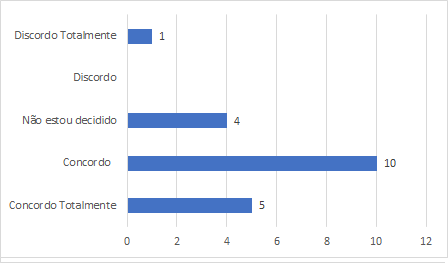
\includegraphics[scale=0.7]{figuras das questoes/6.16.png}
\caption{Respostas questão 6.16}
\end{figure}

\begin{figure}[!t]
\centering
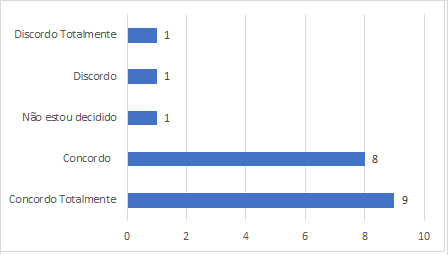
\includegraphics[scale=0.7]{figuras das questoes/6.17.png}
\caption{Respostas questão 6.17}
\end{figure}
\begin{itemize}
%\item Especialista 2: Confirmou-se com o especialista que será realizada a entrevista para examinar a qualidade das perguntas elaboradas com o especialista 1.
\end{itemize}


 

 

 

 \chapter{\label{chap:intro}Conclusão}
 



Com o desenvolvimento deste trabalho, foi possível aquirir um maior conhecimento sobre os conceitos da Segurança da Informação e sobre os requisitos para elaboração de um SGCI que estão presentes na ISO 27001 e sobre os controles e objetivos de controle presentes na ISO 27002.  O TCC em questão é necessário, pois na literatura  \cite{caio2019}, foram encontradas poucas ou nenhuma referência sobre os controles da ISO no contexto de Ecossistema de Software Móvel. O tema ainda é pouco explorado, entretanto a pesquisa se demonstrou viável.
 
O processo metodológico da pesquisa foi longo e desafiador, sendo necessário a leitura de artigos a respeito de metodologia de pesquisa e entrevistas com especialistas. Encontrar especialistas na área de desenvolvimento de dispositivos móveis foi uma tarefa complicada, devido dificuldade de encontrar um profissional com anos de experiência com o mercado. A condução da entrevista foi particularmente desafiador, pois o entrevistado muitas vezes desviava do foco das perguntas a serem feitas, dificultando o processo de identificação da relevâncias das questões levantadas. Um fator limitante para o engajamento de mais participantes na pesquisa pode ter se dado ao tamanho da \textit{survey}, que tinha um tempo médio de resposta de 15 minutos, além do assunto ser relativamente novo e a pesquisa ter sido realizado em uma situação de pandemia.
 
 
Como estudo futuro, podem ser realizadas entrevistas com especialistas, a fim de obter recomendações das questões que ficaram deficitárias de uma resposta forte ou não foram consideradas como preocupação, para que seja possível gerar um guia de boas práticas para auxiliar os desenvolvedores de dispositivos móveis.
 







%----------------------------------------------------------------
% Aqui vai a bibliografia. Existem 3 estilos de citação: use
% 'tcc-alpha' para citações do tipo [Abc+] ou [XYZ] (em ordem
% alfabética na bibliografia), 'tcc-num' para citações
% numéricas do tipo [1], [20], etc., em ordem de referência e
% 'tcc-alpha-full' para citações estilo 'alpha' mas com nomes completos.
%----------------------------------------------------------------
\bibliographystyle{tcc-num}
%\bibliographystyle{tcc-num}
\bibliography{tcc}

%----------------------------------------------------------------
% Após \appendix, se iniciam os capítulos de Apêndice, com
% numeração alfabética.
%----------------------------------------------------------------
%\appendix
%\chapter{Meu primeiro apêndice}
%\chapter{My second appendix}

%----------------------------------------------------------------
% Aqui vão os "capítulos" de anexos. Cada anexo deve
% ser considerado um capítulo.
%----------------------------------------------------------------
%\anexos
%\chapter{Meu primeiro anexo}
%\chapter{My second attachment}

% E aqui (para a felicidade de todos) termina o documento.
\end{document}
